\documentclass[aspectratio=169]{beamer}
\usetheme{ie} % <— this loads beamerthemeie.sty

% If you use minted, compile with: -shell-escape
\usepackage{amsmath, amssymb, mathtools, bm}
\usepackage{graphicx}
\usepackage{tikz}
\usepackage{booktabs}
\usepackage{hyperref}
% \usepackage{minted}
% \setminted{fontsize=\footnotesize, breaklines, autogobble, frame=lines}

\usepackage[backend=biber,style=authoryear,maxbibnames=3]{biblatex}
\addbibresource{references.bib}

% Optional: set short versions for footer
\title[Kolmogorov–Arnold Networks]{KAN Tutorial Slides}
\author[Daniel Precioso \and Francisco Suárez]{Daniel Precioso \and Francisco Suárez}
\date{\today}

\begin{document}
\maketitle

\begin{frame}{Kolmogorov-Arnold Representation Theorem}
Let $ \Omega \subset \mathbb{R}^d $ be a bounded domain and let $ f: \Omega \rightarrow \mathbb{R} $ be a continuous function; i.e. $ f \in C(\Omega) $. Then there exist continuous univariate functions
$$
\Phi_q: \mathbb{R} \to \mathbb{R}, \quad q = 1, \dots, 2d+1;
$$
and continuous univariate functions
$$
\phi_{pq}: \mathbb{R} \to \mathbb{R}, \quad p = 1, \dots, d; \quad q = 1, \dots, 2d+1;
$$
such that for every $\mathbf{x} = (x_1, \dots, x_d) \in \Omega$,
$$
f(\mathbf{x}) = \sum_{q=1}^{2d+1} \Phi_q \left( \sum_{p=1}^d \phi_{pq}(x_p) \right).
$$
\end{frame}

%------------------------------------------

\begin{frame}{Kolmogorov–Arnold Representation Theorem}
	
	\begin{columns}[T,onlytextwidth]
		
		% --- Left column: diagram ---
		\column{0.55\textwidth}
		\centering
		\resizebox{!}{0.75\textheight}{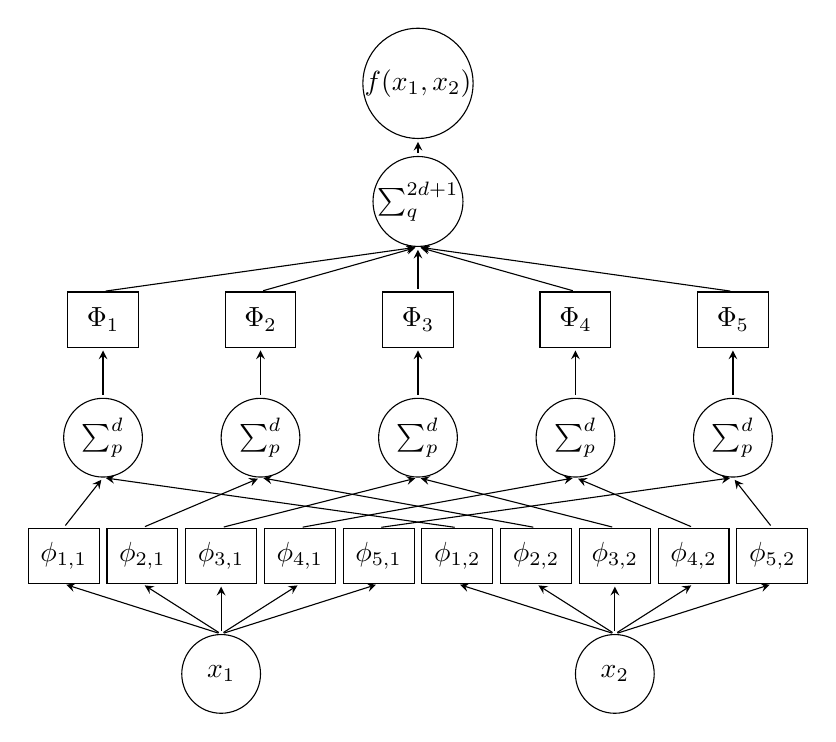
\begin{tikzpicture}[
	neuron/.style={circle, draw, minimum size=10mm, inner sep=0pt},
	box/.style={draw, rectangle, minimum width=9mm, minimum height=7mm, inner sep=1pt, fill=white},
	>=stealth
	]
	
	%-----------------------
	% Customizable heights
	%-----------------------
	\def\hin{0}      % Row 1: inputs
	\def\hphi{1.5}   % Row 2: phi_{i,j} squares
	\def\hsum{3}     % Row 3: per-column sums
	\def\hPhi{4.5}   % Row 4: Phi_j squares
	\def\hsumall{6}  % Row 5: global sum
	\def\hout{7.5}   % Row 6: output
	
	%-----------------------
	% Row 1: inputs
	%-----------------------
	\node[neuron] (X1) at (-2.5,\hin) {$x_1$};
	\node[neuron] (X2) at ( 2.5,\hin) {$x_2$};
	
	%-----------------------
	% Row 2: phi_{i,j} squares
	%-----------------------
	\node[box] (phi1-1) at (-4.5,\hphi) {$\phi_{1,1}$};
	\node[box] (phi2-1) at (-3.5,\hphi) {$\phi_{2,1}$};
	\node[box] (phi3-1) at (-2.5,\hphi) {$\phi_{3,1}$};
	\node[box] (phi4-1) at (-1.5,\hphi) {$\phi_{4,1}$};
	\node[box] (phi5-1) at (-0.5,\hphi) {$\phi_{5,1}$};
	
	\node[box] (phi1-2) at (0.5,\hphi) {$\phi_{1,2}$};
	\node[box] (phi2-2) at (1.5,\hphi) {$\phi_{2,2}$};
	\node[box] (phi3-2) at (2.5,\hphi) {$\phi_{3,2}$};
	\node[box] (phi4-2) at (3.5,\hphi) {$\phi_{4,2}$};
	\node[box] (phi5-2) at (4.5,\hphi) {$\phi_{5,2}$};
	
	%-----------------------
	% Row 3: per-column sums
	%-----------------------
	\node[neuron] (S-1) at (-4,\hsum) {$\textstyle\sum^d_p$};
	\node[neuron] (S-2) at (-2,\hsum) {$\textstyle\sum^d_p$};
	\node[neuron] (S-3) at ( 0,\hsum) {$\textstyle\sum^d_p$};
	\node[neuron] (S-4) at ( 2,\hsum) {$\textstyle\sum^d_p$};
	\node[neuron] (S-5) at ( 4,\hsum) {$\textstyle\sum^d_p$};
	
	%-----------------------
	% Row 4: Phi_j squares
	%-----------------------
	\node[box] (Phi-1) at (-4,\hPhi) {$\Phi_{1}$};
	\node[box] (Phi-2) at (-2,\hPhi) {$\Phi_{2}$};
	\node[box] (Phi-3) at ( 0,\hPhi) {$\Phi_{3}$};
	\node[box] (Phi-4) at ( 2,\hPhi) {$\Phi_{4}$};
	\node[box] (Phi-5) at ( 4,\hPhi) {$\Phi_{5}$};
	
	%-----------------------
	% Row 5: global sum
	%-----------------------
	\node[neuron] (Sall) at (0,\hsumall) {$\textstyle\sum^{2d+1}_q$};
	
	%-----------------------
	% Row 6: output
	%-----------------------
	\node[neuron] (F) at (0,\hout) {$f(x_1,x_2)$};
	
	%-----------------------
	% Connections (use top/bottom anchors)
	%-----------------------
	\tikzset{connect/.style={->,shorten >=1pt,shorten <=1pt}}
	
	% Inputs -> phi (into phi from below)
	\draw[connect] (X1.north) -- (phi1-1.south);
	\draw[connect] (X1.north) -- (phi2-1.south);
	\draw[connect] (X1.north) -- (phi3-1.south);
	\draw[connect] (X1.north) -- (phi4-1.south);
	\draw[connect] (X1.north) -- (phi5-1.south);
	
	\draw[connect] (X2.north) -- (phi1-2.south);
	\draw[connect] (X2.north) -- (phi2-2.south);
	\draw[connect] (X2.north) -- (phi3-2.south);
	\draw[connect] (X2.north) -- (phi4-2.south);
	\draw[connect] (X2.north) -- (phi5-2.south);
	
	% phi -> per-column sums (enter sums from below)
	\draw[connect] (phi1-1.north) -- (S-1.south);
	\draw[connect] (phi1-2.north) -- (S-1.south);
	\draw[connect] (phi2-1.north) -- (S-2.south);
	\draw[connect] (phi2-2.north) -- (S-2.south);
	\draw[connect] (phi3-1.north) -- (S-3.south);
	\draw[connect] (phi3-2.north) -- (S-3.south);
	\draw[connect] (phi4-1.north) -- (S-4.south);
	\draw[connect] (phi4-2.north) -- (S-4.south);
	\draw[connect] (phi5-1.north) -- (S-5.south);
	\draw[connect] (phi5-2.north) -- (S-5.south);
	
	% sums -> Phi (upwards)
	\draw[connect] (S-1.north) -- (Phi-1.south);
	\draw[connect] (S-2.north) -- (Phi-2.south);
	\draw[connect] (S-3.north) -- (Phi-3.south);
	\draw[connect] (S-4.north) -- (Phi-4.south);
	\draw[connect] (S-5.north) -- (Phi-5.south);
	
	% Phi -> global sum
	\draw[connect] (Phi-1.north) -- (Sall.south);
	\draw[connect] (Phi-2.north) -- (Sall.south);
	\draw[connect] (Phi-3.north) -- (Sall.south);
	\draw[connect] (Phi-4.north) -- (Sall.south);
	\draw[connect] (Phi-5.north) -- (Sall.south);
	
	% Global sum -> output
	\draw[connect] (Sall.north) -- (F.south);
	
\end{tikzpicture}}
		
		% --- Right column: explanation ---
		\column{0.4\textwidth}
		The theorem states that any $f(x_1, x_2)$ can be written as a sum of univariate compositions.
		
		The diagram shows this expression visually: each block represents a component of the decomposition.
		
		Together, they form a \textbf{Kolmogorov–Arnold Network (KAN)}.
		
	\end{columns}
	
\end{frame}

%------------------------------------------

\begin{frame}{Kolmogorov–Arnold Networks}
	
	\begin{columns}[T,onlytextwidth]
		
		% --- Left column: diagram ---
		\column{0.55\textwidth}
		\centering
		\resizebox{!}{0.8\textheight}{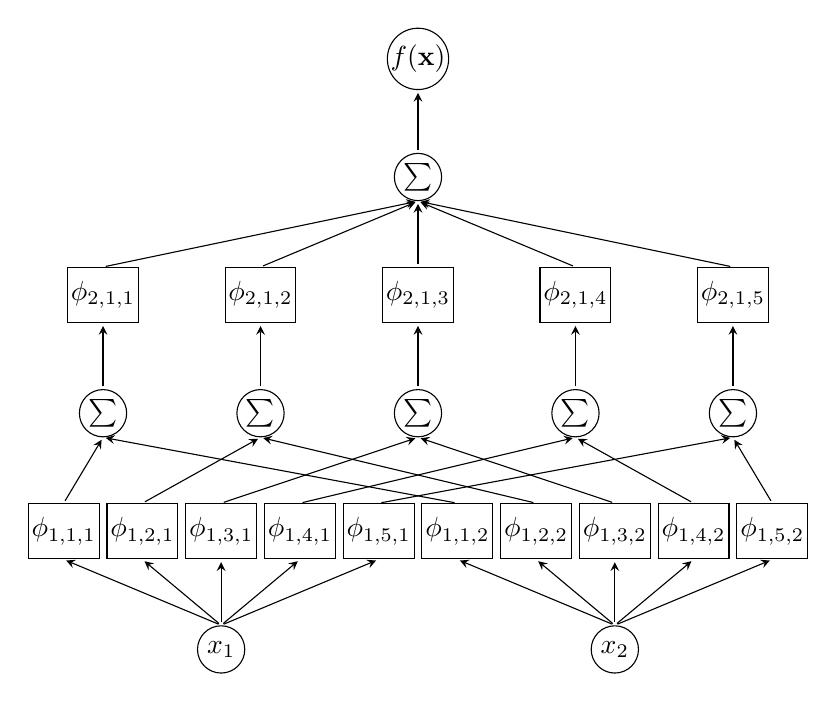
\begin{tikzpicture}[
	neuron/.style={circle, draw, minimum size=6mm, inner sep=0pt},
	box/.style={draw, rectangle, minimum width=9mm, minimum height=7mm, inner sep=1pt, fill=white},
	>=stealth
	]
	
	%-----------------------
	% Customizable heights
	%-----------------------
	\def\hin{0}      % Row 1: inputs
	\def\hphi{1.5}   % Row 2: phi_{i,j} squares
	\def\hsum{3}     % Row 3: per-column sums
	\def\hPhi{4.5}   % Row 4: Phi_j squares
	\def\hsumall{6}  % Row 5: global sum
	\def\hout{7.5}   % Row 6: output
	
	%-----------------------
	% Row 1: inputs
	%-----------------------
	\node[neuron] (X1) at (-2.5,\hin) {$x_1$};
	\node[neuron] (X2) at ( 2.5,\hin) {$x_2$};
	
	%-----------------------
	% Row 2: phi_{i,j} squares
	%-----------------------
	\node[box] (phi111) at (-4.5,\hphi) {$\phi_{1,1,1}$};
	\node[box] (phi121) at (-3.5,\hphi) {$\phi_{1,2,1}$};
	\node[box] (phi131) at (-2.5,\hphi) {$\phi_{1,3,1}$};
	\node[box] (phi141) at (-1.5,\hphi) {$\phi_{1,4,1}$};
	\node[box] (phi151) at (-0.5,\hphi) {$\phi_{1,5,1}$};
	
	\node[box] (phi112) at (0.5,\hphi) {$\phi_{1,1,2}$};
	\node[box] (phi122) at (1.5,\hphi) {$\phi_{1,2,2}$};
	\node[box] (phi132) at (2.5,\hphi) {$\phi_{1,3,2}$};
	\node[box] (phi142) at (3.5,\hphi) {$\phi_{1,4,2}$};
	\node[box] (phi152) at (4.5,\hphi) {$\phi_{1,5,2}$};
	
	%-----------------------
	% Row 3: per-column sums
	%-----------------------
	\node[neuron] (S-1) at (-4,\hsum) {$\textstyle\sum$};
	\node[neuron] (S-2) at (-2,\hsum) {$\textstyle\sum$};
	\node[neuron] (S-3) at ( 0,\hsum) {$\textstyle\sum$};
	\node[neuron] (S-4) at ( 2,\hsum) {$\textstyle\sum$};
	\node[neuron] (S-5) at ( 4,\hsum) {$\textstyle\sum$};
	
	%-----------------------
	% Row 4: Phi_j squares
	%-----------------------
	\node[box] (phi211) at (-4,\hPhi) {$\phi_{2,1,1}$};
	\node[box] (phi212) at (-2,\hPhi) {$\phi_{2,1,2}$};
	\node[box] (phi213) at ( 0,\hPhi) {$\phi_{2,1,3}$};
	\node[box] (phi214) at ( 2,\hPhi) {$\phi_{2,1,4}$};
	\node[box] (phi215) at ( 4,\hPhi) {$\phi_{2,1,5}$};
	
	%-----------------------
	% Row 5: global sum
	%-----------------------
	\node[neuron] (Sall) at (0,\hsumall) {$\textstyle\sum$};
	
	%-----------------------
	% Row 6: output
	%-----------------------
	\node[neuron] (F) at (0,\hout) {$f(\mathbf{x})$};
	
	%-----------------------
	% Connections (use top/bottom anchors)
	%-----------------------
	\tikzset{connect/.style={->,shorten >=1pt,shorten <=1pt}}
	
	% Inputs -> phi (into phi from below)
	\draw[connect] (X1.north) -- (phi111.south);
	\draw[connect] (X1.north) -- (phi121.south);
	\draw[connect] (X1.north) -- (phi131.south);
	\draw[connect] (X1.north) -- (phi141.south);
	\draw[connect] (X1.north) -- (phi151.south);
	
	\draw[connect] (X2.north) -- (phi112.south);
	\draw[connect] (X2.north) -- (phi122.south);
	\draw[connect] (X2.north) -- (phi132.south);
	\draw[connect] (X2.north) -- (phi142.south);
	\draw[connect] (X2.north) -- (phi152.south);
	
	% phi -> per-column sums (enter sums from below)
	\draw[connect] (phi111.north) -- (S-1.south);
	\draw[connect] (phi112.north) -- (S-1.south);
	\draw[connect] (phi121.north) -- (S-2.south);
	\draw[connect] (phi122.north) -- (S-2.south);
	\draw[connect] (phi131.north) -- (S-3.south);
	\draw[connect] (phi132.north) -- (S-3.south);
	\draw[connect] (phi141.north) -- (S-4.south);
	\draw[connect] (phi142.north) -- (S-4.south);
	\draw[connect] (phi151.north) -- (S-5.south);
	\draw[connect] (phi152.north) -- (S-5.south);
	
	% sums -> Phi (upwards)
	\draw[connect] (S-1.north) -- (phi211.south);
	\draw[connect] (S-2.north) -- (phi212.south);
	\draw[connect] (S-3.north) -- (phi213.south);
	\draw[connect] (S-4.north) -- (phi214.south);
	\draw[connect] (S-5.north) -- (phi215.south);
	
	% Phi -> global sum
	\draw[connect] (phi211.north) -- (Sall.south);
	\draw[connect] (phi212.north) -- (Sall.south);
	\draw[connect] (phi213.north) -- (Sall.south);
	\draw[connect] (phi214.north) -- (Sall.south);
	\draw[connect] (phi215.north) -- (Sall.south);
	
	% Global sum -> output
	\draw[connect] (Sall.north) -- (F.south);
	
\end{tikzpicture}}
		
		% --- Right column: explanation ---
		\column{0.4\textwidth}
		In a network setting, each univariate function is written as $\phi_{d,p,q}$, where:
		\vspace{0.8em}
		\begin{itemize}
			\item $d$: layer depth  
			\item $p$: output node index  
			\item $q$: input node index
		\end{itemize}
		
		\vspace{1em}
		This network is a \textbf{KAN [2,5,1]}:\\it has 2 inputs, one hidden layer with 5 nodes, and 1 output.
		
	\end{columns}
	
\end{frame}

%------------------------------------------

\begin{frame}{Kolmogorov–Arnold Networks}
	\begin{columns}[T,onlytextwidth]
		
		% --- Left column: diagram ---
		\column{0.5\textwidth}
		\centering
		\resizebox{!}{0.8\textheight}{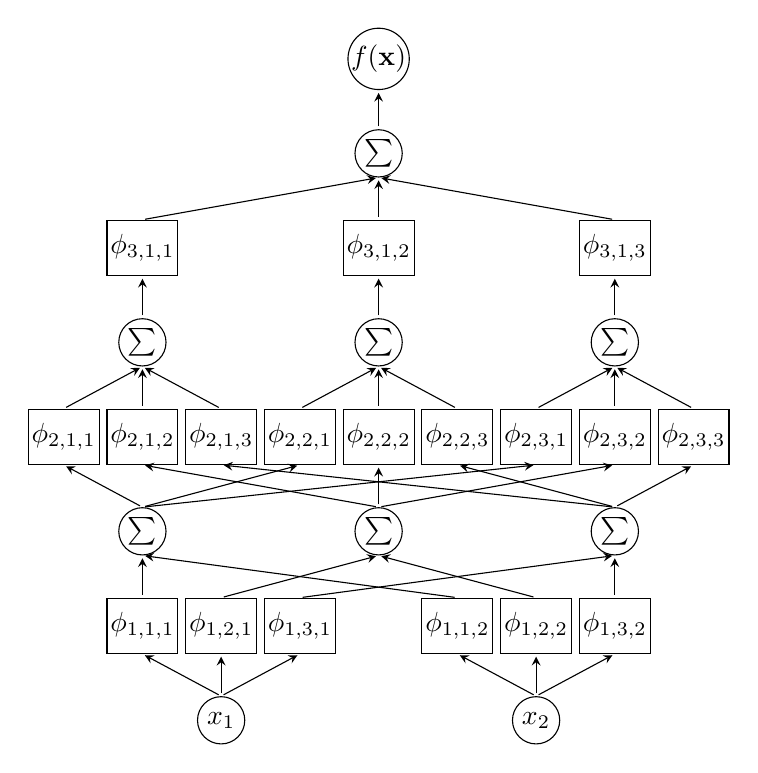
\begin{tikzpicture}[
	neuron/.style={circle, draw, minimum size=6mm, inner sep=0pt},
	box/.style={draw, rectangle, minimum width=9mm, minimum height=7mm, inner sep=1pt, fill=white},
	>=stealth
	]
	
	%-----------------------
	% Customizable heights (compact stack)
	%-----------------------
	\def\hin{0.0}        % inputs
	\def\hphiI{1.2}      % layer-1 phi_{1,p,q}
	\def\hsumI{2.4}      % first hidden sums (S1..S3)
	\def\hphiII{3.6}     % layer-2 phi_{2,r,q} (9 boxes)
	\def\hsumII{4.8}     % second hidden sums (T1..T3)
	\def\hphiIII{6.0}    % layer-3 phi_{3,1,r}
	\def\hsumall{7.2}    % global sum
	\def\hout{8.4}       % output
	
	%-----------------------
	% Row 1: inputs
	%-----------------------
	\node[neuron] (X1) at (-2,\hin) {$x_1$};
	\node[neuron] (X2) at ( 2,\hin) {$x_2$};
	
	%-----------------------
	% Row 2: layer-1 univariate functions phi_{1,p,q}
	% columns p=1..3 placed at xA,xB,xC; q=1 from x1 (left), q=2 from x2 (right)
	\node[box] (phi111) at (-3,\hphiI) {$\phi_{1,1,1}$};
	\node[box] (phi121) at (-2,\hphiI) {$\phi_{1,2,1}$};
	\node[box] (phi131) at (-1,\hphiI) {$\phi_{1,3,1}$};
	
	\node[box] (phi112) at (1,\hphiI) {$\phi_{1,1,2}$};
	\node[box] (phi122) at (2,\hphiI) {$\phi_{1,2,2}$};
	\node[box] (phi132) at (3,\hphiI) {$\phi_{1,3,2}$};
	
	%-----------------------
	% Row 3: first hidden sums S1..S3 (p = 1..3)
	%-----------------------
	\node[neuron] (S1) at (-3,\hsumI) {$\textstyle\sum$};
	\node[neuron] (S2) at (0,\hsumI) {$\textstyle\sum$};
	\node[neuron] (S3) at (3,\hsumI) {$\textstyle\sum$};
	
	%-----------------------
	% Row 4: layer-2 univariate functions phi_{2,r,q}
	% For each target r∈{1,2,3} (columns xA,xB,xC), we place three boxes fed by S1,S2,S3.
	% left/mid/right offsets correspond to q=1 from S1, q=2 from S2, q=3 from S3.
	\node[box] (phi211) at (-4,\hphiII) {$\phi_{2,1,1}$};
	\node[box] (phi221) at (-3,     \hphiII) {$\phi_{2,1,2}$};
	\node[box] (phi231) at (-2,\hphiII) {$\phi_{2,1,3}$};
	
	\node[box] (phi212) at (-1,\hphiII) {$\phi_{2,2,1}$};
	\node[box] (phi222) at (0,     \hphiII) {$\phi_{2,2,2}$};
	\node[box] (phi232) at (1,\hphiII) {$\phi_{2,2,3}$};
	
	\node[box] (phi213) at (2,\hphiII) {$\phi_{2,3,1}$};
	\node[box] (phi223) at (3,     \hphiII) {$\phi_{2,3,2}$};
	\node[box] (phi233) at (4,\hphiII) {$\phi_{2,3,3}$};
	
	%-----------------------
	% Row 5: second hidden sums T1..T3 (r = 1..3)
	%-----------------------
	\node[neuron] (T1) at (-3,\hsumII) {$\textstyle\sum$};
	\node[neuron] (T2) at (0,\hsumII) {$\textstyle\sum$};
	\node[neuron] (T3) at (3,\hsumII) {$\textstyle\sum$};
	
	%-----------------------
	% Row 6: layer-3 univariate functions phi_{3,1,r} (r feeds the single top unit)
	%-----------------------
	\node[box] (phi311) at (-3,\hphiIII) {$\phi_{3,1,1}$};
	\node[box] (phi312) at (0,\hphiIII) {$\phi_{3,1,2}$};
	\node[box] (phi313) at (3,\hphiIII) {$\phi_{3,1,3}$};
	
	%-----------------------
	% Row 7: global sum and Row 8: output
	%-----------------------
	\node[neuron] (Sall) at (0,\hsumall) {$\textstyle\sum$};
	\node[neuron] (F)    at (0,\hout)    {$f(\mathbf{x})$};
	
	%-----------------------
	% Connections (top/bottom anchors)
	%-----------------------
	\tikzset{connect/.style={->,shorten >=1pt,shorten <=1pt}}
	
	% Inputs -> layer-1 phi
	\draw[connect] (X1.north) -- (phi111.south);
	\draw[connect] (X1.north) -- (phi121.south);
	\draw[connect] (X1.north) -- (phi131.south);
	
	\draw[connect] (X2.north) -- (phi112.south);
	\draw[connect] (X2.north) -- (phi122.south);
	\draw[connect] (X2.north) -- (phi132.south);
	
	% layer-1 phi -> first hidden sums
	\draw[connect] (phi111.north) -- (S1.south);
	\draw[connect] (phi112.north) -- (S1.south);
	
	\draw[connect] (phi121.north) -- (S2.south);
	\draw[connect] (phi122.north) -- (S2.south);
	
	\draw[connect] (phi131.north) -- (S3.south);
	\draw[connect] (phi132.north) -- (S3.south);
	
	% first hidden sums S{1,2,3} -> layer-2 phi boxes for each target T{1,2,3}
	% Column r=1 (xA)
	\draw[connect] (S1.north) -- (phi211.south);
	\draw[connect] (S2.north) -- (phi221.south);
	\draw[connect] (S3.north) -- (phi231.south);
	% Column r=2 (xB)
	\draw[connect] (S1.north) -- (phi212.south);
	\draw[connect] (S2.north) -- (phi222.south);
	\draw[connect] (S3.north) -- (phi232.south);
	% Column r=3 (xC)
	\draw[connect] (S1.north) -- (phi213.south);
	\draw[connect] (S2.north) -- (phi223.south);
	\draw[connect] (S3.north) -- (phi233.south);
	
	% layer-2 phi -> second hidden sums T{1,2,3}
	\draw[connect] (phi211.north) -- (T1.south);
	\draw[connect] (phi221.north) -- (T1.south);
	\draw[connect] (phi231.north) -- (T1.south);
	
	\draw[connect] (phi212.north) -- (T2.south);
	\draw[connect] (phi222.north) -- (T2.south);
	\draw[connect] (phi232.north) -- (T2.south);
	
	\draw[connect] (phi213.north) -- (T3.south);
	\draw[connect] (phi223.north) -- (T3.south);
	\draw[connect] (phi233.north) -- (T3.south);
	
	% layer-3 phi -> global sum
	\draw[connect] (T1.north) -- (phi311.south);
	\draw[connect] (T2.north) -- (phi312.south);
	\draw[connect] (T3.north) -- (phi313.south);
	
	\draw[connect] (phi311.north) -- (Sall.south);
	\draw[connect] (phi312.north) -- (Sall.south);
	\draw[connect] (phi313.north) -- (Sall.south);
	
	% Global sum -> output
	\draw[connect] (Sall.north) -- (F.south);
	
\end{tikzpicture}
}
		
		% --- Right column: explanation ---
		\column{0.45\textwidth}
		\textbf{KAN [2,3,3,1]}: 2 inputs, two hidden layers of 3, 1 output.
		
		\vspace{0.8em}
		\textit{Why go deeper?}
		\begin{itemize}
			\item \textbf{Theory:} Any continuous $f(\mathbf{x})$ admits a shallow KAN $[I,\,2\ I + 1,\,1]$.
			\item \textbf{Practice:} Deeper KANs can model non-continuous functions. Depth improves expressivity.
		\end{itemize}
		
	\end{columns}
\end{frame}

%------------------------------------------

\begin{frame}{B-Splines}
	$\phi_{d,p,q}$ can be chosen from any family of continuous univariate functions. A common choice is the \textbf{B-spline} family.
	
	A B-spline of $k$-order is defined as:
	
	$$B_k(x) = \sum_{i=0}^{G+k-1} P_i N_{i,k}(x)$$
	
	where $G$ is the number of segments (grid size),\\
	$N_{i,k}(x)$ are the basis functions of $k$-order (for a total of $G+k$),\\
	and $P_i$ are the control points coefficients (spline weights).
\end{frame}

%------------------------------------------

\begin{frame}{B-Splines - Basis Function}
The basis functions follow the standard \textbf{Cox–de Boor recursive definition}:

\begin{flalign*}
	N_{i,0}(x) &= 
	\begin{cases}
		1, & t_{i-k} \le x < t_{i-k+1},\\
		0, & \text{otherwise}
	\end{cases} &
\end{flalign*}

\begin{flalign*}
	N_{i,k}(x) &=
	\frac{x - t_{i-k}}{t_{i} - t_{i-k}} N_{i,k-1}(x)
	+
	\frac{t_{i+1} - x}{t_{i+1} - t_{i-k+1}} N_{i,k-1}(x),
	\quad k > 0,&
\end{flalign*}

where $\mathbf{t}$ is the \textbf{knot vector}, a non-decreasing sequence of real numbers of length $(G + 2k + 1)$, being $\mathbf{t} = (t_{-k}, \dots, t_0, \dots, t_G, \dots t_{G+k})$.
\end{frame}

%------------------------------------------

\begin{frame}{B-Splines - Knot Vector}
	
	\begin{columns}[T,onlytextwidth]
		
		% --- Left column ---
		\column{0.45\textwidth}
		
		Knot vector $\mathbf{t}$ with
		$$a=t_{-k},\quad b=t_{G+k}$$
		Clamped uniform knots on $[a,b]$:
		\begin{align*}
			t_{-k} &=\cdots=t_{0}=a,\\
			t_{G} &=\cdots=t_{G+k}=b,\\
			t_{j} &= a+\frac{j}{G}(b-a),\quad j=0,\dots,G\\
		\end{align*}
		
		% --- Right column ---
		\column{0.5\textwidth}
		\begin{figure}
			\centering
			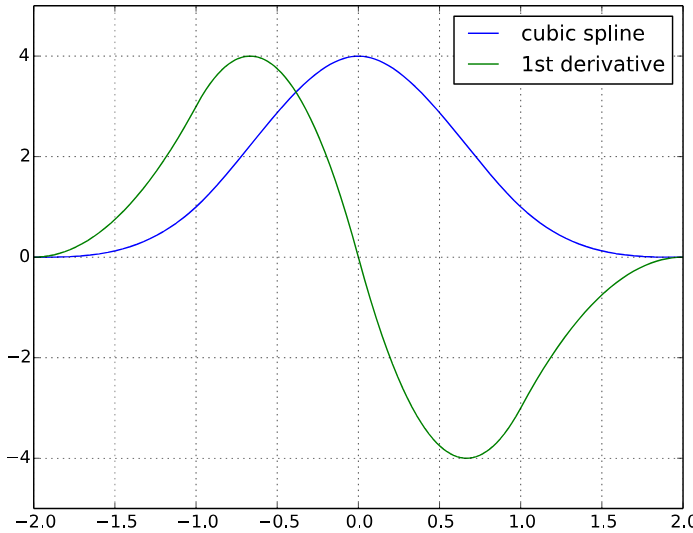
\includegraphics[height=0.6\textheight]{../images/Cardinal_cubic_B-spline2.png}
		\end{figure}
		$\mathbf{t}=(-2, -2, -2, -2, -1, 0, 1, 2, 2, 2, 2)$\\
		$\mathbf{P}=(0, 0, 0, 6, 0, 0, 0)$
		
	\end{columns}
	
\end{frame}

%------------------------------------------

\begin{frame}{B-Splines as KAN Edges}
	
	All univariate functions share the same spline degree $k$ and number of control points $n$.  
	Each $\phi_{d,p,q}$ combines a basis function (similar to residual connections) with a B-spline expansion:
	
	\begin{flalign*}
		\phi(x) = w_b\, b(x) + w_s \sum_{i=0}^{G+k-1} P_i\, N_{i,k}(x)
	\end{flalign*}
	
	Here, $w_b$ is the learnable weight of the basis function, $w_s$ is the weight for the spline, and the control point coefficients $P_i$ scale the individual B-spline functions directly. We choose the basis as:
	
	\begin{flalign*}
		b(x) = \mathrm{SiLU}(x) = \frac{x}{1 + e^{-x}}
	\end{flalign*}
	
\end{frame}

%------------------------------------------

\begin{frame}{KAN Parameters}
	
	\begin{columns}[T,onlytextwidth]
		
		% --- Left column: diagram ---
		\column{0.5\textwidth}
		\centering
		\resizebox{!}{0.8\textheight}{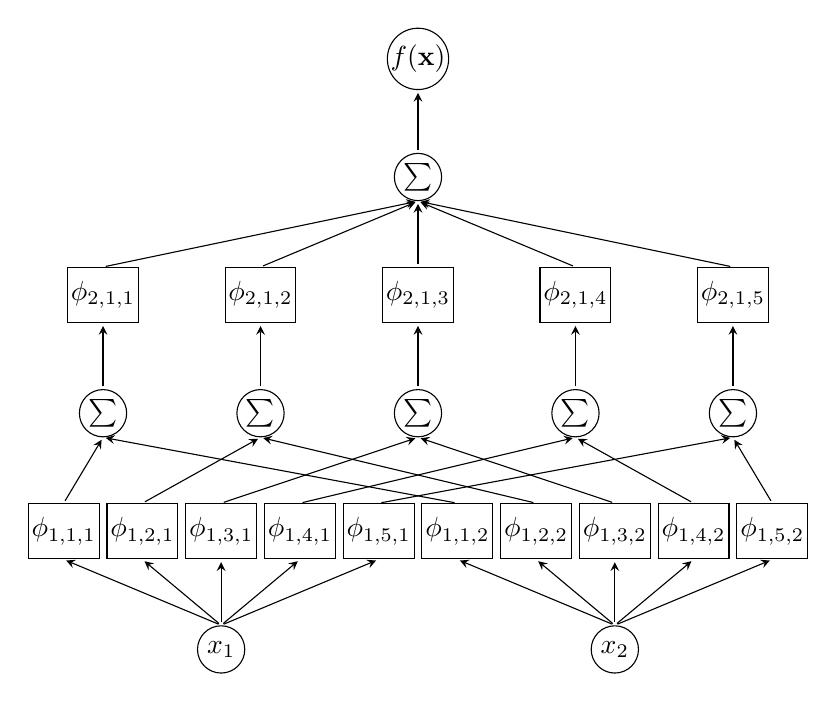
\begin{tikzpicture}[
	neuron/.style={circle, draw, minimum size=6mm, inner sep=0pt},
	box/.style={draw, rectangle, minimum width=9mm, minimum height=7mm, inner sep=1pt, fill=white},
	>=stealth
	]
	
	%-----------------------
	% Customizable heights
	%-----------------------
	\def\hin{0}      % Row 1: inputs
	\def\hphi{1.5}   % Row 2: phi_{i,j} squares
	\def\hsum{3}     % Row 3: per-column sums
	\def\hPhi{4.5}   % Row 4: Phi_j squares
	\def\hsumall{6}  % Row 5: global sum
	\def\hout{7.5}   % Row 6: output
	
	%-----------------------
	% Row 1: inputs
	%-----------------------
	\node[neuron] (X1) at (-2.5,\hin) {$x_1$};
	\node[neuron] (X2) at ( 2.5,\hin) {$x_2$};
	
	%-----------------------
	% Row 2: phi_{i,j} squares
	%-----------------------
	\node[box] (phi111) at (-4.5,\hphi) {$\phi_{1,1,1}$};
	\node[box] (phi121) at (-3.5,\hphi) {$\phi_{1,2,1}$};
	\node[box] (phi131) at (-2.5,\hphi) {$\phi_{1,3,1}$};
	\node[box] (phi141) at (-1.5,\hphi) {$\phi_{1,4,1}$};
	\node[box] (phi151) at (-0.5,\hphi) {$\phi_{1,5,1}$};
	
	\node[box] (phi112) at (0.5,\hphi) {$\phi_{1,1,2}$};
	\node[box] (phi122) at (1.5,\hphi) {$\phi_{1,2,2}$};
	\node[box] (phi132) at (2.5,\hphi) {$\phi_{1,3,2}$};
	\node[box] (phi142) at (3.5,\hphi) {$\phi_{1,4,2}$};
	\node[box] (phi152) at (4.5,\hphi) {$\phi_{1,5,2}$};
	
	%-----------------------
	% Row 3: per-column sums
	%-----------------------
	\node[neuron] (S-1) at (-4,\hsum) {$\textstyle\sum$};
	\node[neuron] (S-2) at (-2,\hsum) {$\textstyle\sum$};
	\node[neuron] (S-3) at ( 0,\hsum) {$\textstyle\sum$};
	\node[neuron] (S-4) at ( 2,\hsum) {$\textstyle\sum$};
	\node[neuron] (S-5) at ( 4,\hsum) {$\textstyle\sum$};
	
	%-----------------------
	% Row 4: Phi_j squares
	%-----------------------
	\node[box] (phi211) at (-4,\hPhi) {$\phi_{2,1,1}$};
	\node[box] (phi212) at (-2,\hPhi) {$\phi_{2,1,2}$};
	\node[box] (phi213) at ( 0,\hPhi) {$\phi_{2,1,3}$};
	\node[box] (phi214) at ( 2,\hPhi) {$\phi_{2,1,4}$};
	\node[box] (phi215) at ( 4,\hPhi) {$\phi_{2,1,5}$};
	
	%-----------------------
	% Row 5: global sum
	%-----------------------
	\node[neuron] (Sall) at (0,\hsumall) {$\textstyle\sum$};
	
	%-----------------------
	% Row 6: output
	%-----------------------
	\node[neuron] (F) at (0,\hout) {$f(\mathbf{x})$};
	
	%-----------------------
	% Connections (use top/bottom anchors)
	%-----------------------
	\tikzset{connect/.style={->,shorten >=1pt,shorten <=1pt}}
	
	% Inputs -> phi (into phi from below)
	\draw[connect] (X1.north) -- (phi111.south);
	\draw[connect] (X1.north) -- (phi121.south);
	\draw[connect] (X1.north) -- (phi131.south);
	\draw[connect] (X1.north) -- (phi141.south);
	\draw[connect] (X1.north) -- (phi151.south);
	
	\draw[connect] (X2.north) -- (phi112.south);
	\draw[connect] (X2.north) -- (phi122.south);
	\draw[connect] (X2.north) -- (phi132.south);
	\draw[connect] (X2.north) -- (phi142.south);
	\draw[connect] (X2.north) -- (phi152.south);
	
	% phi -> per-column sums (enter sums from below)
	\draw[connect] (phi111.north) -- (S-1.south);
	\draw[connect] (phi112.north) -- (S-1.south);
	\draw[connect] (phi121.north) -- (S-2.south);
	\draw[connect] (phi122.north) -- (S-2.south);
	\draw[connect] (phi131.north) -- (S-3.south);
	\draw[connect] (phi132.north) -- (S-3.south);
	\draw[connect] (phi141.north) -- (S-4.south);
	\draw[connect] (phi142.north) -- (S-4.south);
	\draw[connect] (phi151.north) -- (S-5.south);
	\draw[connect] (phi152.north) -- (S-5.south);
	
	% sums -> Phi (upwards)
	\draw[connect] (S-1.north) -- (phi211.south);
	\draw[connect] (S-2.north) -- (phi212.south);
	\draw[connect] (S-3.north) -- (phi213.south);
	\draw[connect] (S-4.north) -- (phi214.south);
	\draw[connect] (S-5.north) -- (phi215.south);
	
	% Phi -> global sum
	\draw[connect] (phi211.north) -- (Sall.south);
	\draw[connect] (phi212.north) -- (Sall.south);
	\draw[connect] (phi213.north) -- (Sall.south);
	\draw[connect] (phi214.north) -- (Sall.south);
	\draw[connect] (phi215.north) -- (Sall.south);
	
	% Global sum -> output
	\draw[connect] (Sall.north) -- (F.south);
	
\end{tikzpicture}}
		
		% --- Right column: explanation ---
		\column{0.45\textwidth}
		
		\textbf{Hyperparameters}
		\begin{itemize}
			\item $G$: grid size (no. intervals).
			\item $k$: B-spline order.
		\end{itemize}
		
		\vspace{0.8em}
		\textbf{Learnable parameters}\\(for each edge)
		\begin{itemize}
			\item $P_i$: control points, $i \in [0, G+k-1]$.
			\item $w_b$: basis weight.
			\item $w_s$: spline weight.
		\end{itemize}
		
	\end{columns}
	
\end{frame}

%------------------------------------------

\begin{frame}{KAN Backpropagation}
	Loss function is L2 (RMSE): 
	
	\begin{equation*}
		L = \left\| y - \hat{y} \right\|_2 = \left\| f(\mathbf{x}) - \hat{f}_{d}(\mathbf{x}) \right\|_2 = \left\| f(\mathbf{x}) - \sum_q \phi_{d,q}(\mathbf{x}) \right\|_2
	\end{equation*}
	
	Where $d$ is the last layer, and $p=1$ because we have a single output. The coefficients of that layer are $P_{d,q,i}$.
	
	\begin{equation*}
		\frac{\partial L}{\partial P_{d,q,i}} = \frac{\partial L}{\partial \hat{f}_{d}(\mathbf{x})} \cdot \frac{\partial \hat{f}_{d}(\mathbf{x})}{\partial P_{d,q,i}} 
	\end{equation*}
	
	And for the previous layer $d-1$:
	
	\begin{equation*}
		\frac{\partial L}{\partial P_{d-1,p,q,i}} = \frac{\partial L}{\partial \hat{f}_{d}(\mathbf{x})} \cdot \frac{\partial \hat{f}_{d}(\mathbf{x})}{\partial \hat{f}_{d-1,p}(\mathbf{x})} \cdot \frac{\partial \hat{f}_{d-1,p}(\mathbf{x})}{\partial P_{d-1,p,q,i}} 
	\end{equation*}
	
\end{frame}

%------------------------------------------

\begin{frame}{Capabilities of KANs with B-Splines}
	
	\begin{itemize}
		\item \textbf{Grid extension}: progressively increase model capacity by refining the spline grid without retraining from scratch.
		\item \textbf{Continual learning}: local support ensures new information affects only nearby regions, reducing catastrophic forgetting.
		\item \textbf{Sparsity}: regularization and pruning remove redundant components, simplifying the model without major accuracy loss.
		\item \textbf{Symbolic regression}: univariate structure enables conversion of learned functions into interpretable closed-form expressions.
	\end{itemize}
	
\end{frame}

%------------------------------------------

\begin{frame}{Capabilities - Grid Extension}
	\begin{columns}[T,onlytextwidth]
		
		% --- Left column: explanation ---
		\column{0.6\textwidth}
		\textbf{Grid extension} refines a trained KAN by adding more spline knots without restarting training.
		
		\begin{itemize}
			\item Train on a coarse grid first.
			\item Add intervals to increase resolution and capacity (increase $G$)
			\item Initialize new coefficients ($P_i$) by least-squares fitting.
			\item Continue training to improve accuracy.
		\end{itemize}
		
		Test loss often improves until the parameter count roughly matches the number of data points.
		
		% --- Right column: image ---
		\column{0.4\textwidth}
		\centering
		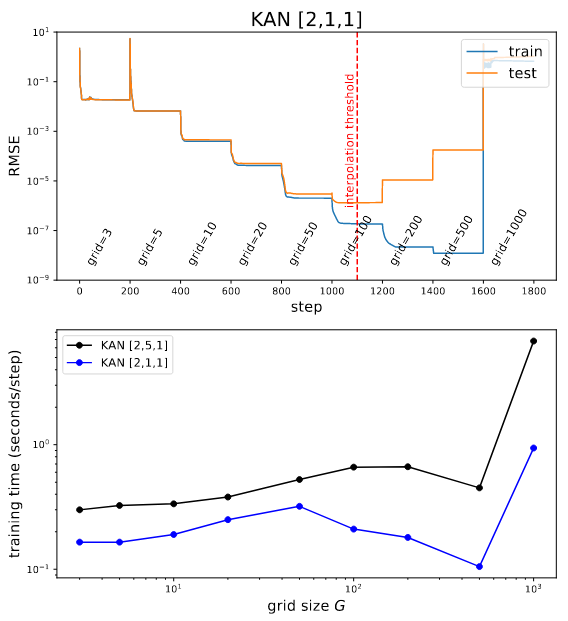
\includegraphics[height=0.8\textheight]{../images/grid_extension.png}
		
	\end{columns}
\end{frame}

%------------------------------------------

\begin{frame}{Capabilities - Continual Learning}
	
	Because B-splines have \textbf{local support}, updates to $\phi(x)$ in one region of the input space affect only nearby points.  
	This locality mitigates \textbf{catastrophic forgetting}, a common issue in MLPs where learning new data can overwrite previously acquired knowledge.
	
	\begin{figure}
		\centering
		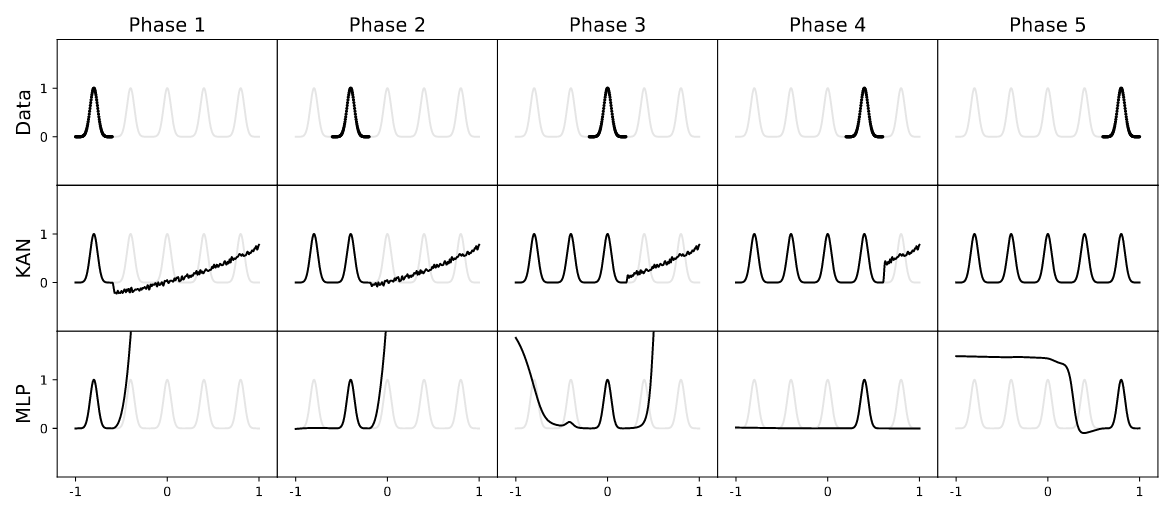
\includegraphics[height=0.6\textheight]{../images/continual_learning.png}
	\end{figure}
	
\end{frame}


%------------------------------------------

\begin{frame}{Capabilities - Sparsity}
	\begin{columns}[T,onlytextwidth]
		
		% --- Left column: explanation ---
		\column{0.55\textwidth}
		
		\textbf{Sparsity} removes unnecessary components, revealing the essential structure of our target function.
		
		\vspace{0.6em}
		\begin{itemize}
			\item \textbf{Regularization} drives many spline weights toward zero.
			\item Irrelevant edges can be pruned after training.
			\item The result is a compact, interpretable network.
		\end{itemize}
		
		Sparsity helps towards \textbf{interpretability}.
		
		% --- Right column: diagram ---
		\column{0.4\textwidth}
		\centering
		\resizebox{!}{0.65\textheight}{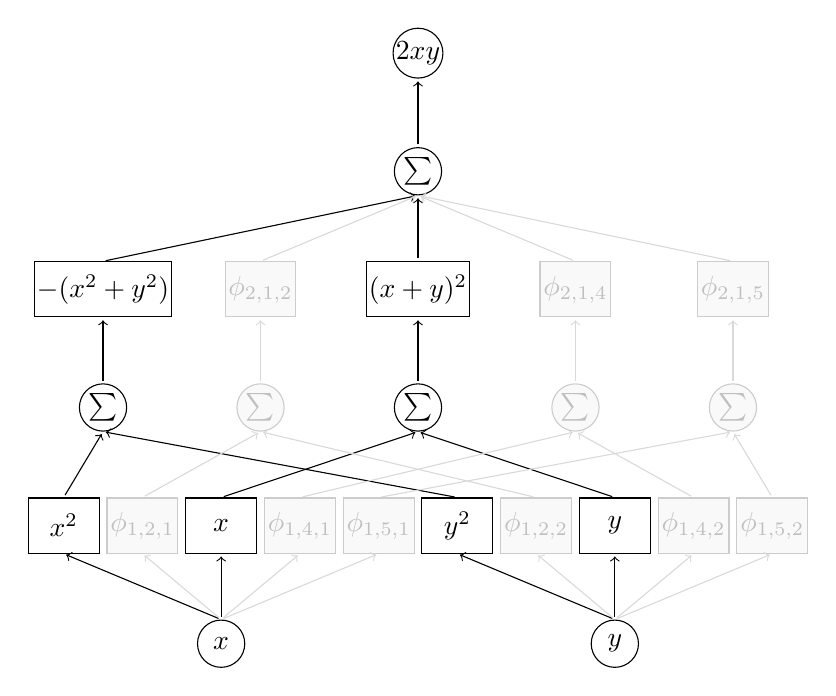
\begin{tikzpicture}[
	neuron/.style={circle, draw, minimum size=6mm, inner sep=0pt},
	box/.style={draw, rectangle, minimum width=9mm, minimum height=7mm, inner sep=1pt},
	faded/.style={draw=gray!40, fill=gray!5, text=gray!50},
	fadedline/.style={->, shorten >=1pt, shorten <=1pt, draw=gray!30},
	]
	
	%-----------------------
	% Customizable heights
	%-----------------------
	\def\hin{0}
	\def\hphi{1.5}
	\def\hsum{3}
	\def\hPhi{4.5}
	\def\hsumall{6}
	\def\hout{7.5}
	
	%-----------------------
	% Row 1: inputs
	%-----------------------
	\node[neuron] (X1) at (-2.5,\hin) {$x$};
	\node[neuron] (X2) at ( 2.5,\hin) {$y$};
	
	%-----------------------
	% Row 2: phi_{i,j} squares
	%-----------------------
	\node[box] (phi111) at (-4.5,\hphi) {$x^2$}; % active
	\node[box] (phi121) [faded] at (-3.5,\hphi) {$\phi_{1,2,1}$}; % faded
	\node[box] (phi131) at (-2.5,\hphi) {$x$}; % active
	\node[box] (phi141) [faded] at (-1.5,\hphi) {$\phi_{1,4,1}$}; % faded
	\node[box] (phi151) [faded] at (-0.5,\hphi) {$\phi_{1,5,1}$}; % faded
	
	\node[box] (phi112) at (0.5,\hphi) {$y^2$}; % active
	\node[box] (phi122) [faded] at (1.5,\hphi) {$\phi_{1,2,2}$}; % faded
	\node[box] (phi132) at (2.5,\hphi) {$y$}; % active
	\node[box] (phi142) [faded] at (3.5,\hphi) {$\phi_{1,4,2}$}; % faded
	\node[box] (phi152) [faded] at (4.5,\hphi) {$\phi_{1,5,2}$}; % faded
	
	%-----------------------
	% Row 3: per-column sums
	%-----------------------
	\node[neuron] (S-1) at (-4,\hsum) {$\sum$};
	\node[neuron] (S-2) [faded] at (-2,\hsum) {$\sum$};
	\node[neuron] (S-3) at ( 0,\hsum) {$\sum$};
	\node[neuron] (S-4) [faded] at ( 2,\hsum) {$\sum$};
	\node[neuron] (S-5) [faded] at ( 4,\hsum) {$\sum$};
	
	%-----------------------
	% Row 4: Phi_j squares
	%-----------------------
	\node[box] (phi211) at (-4,\hPhi) {$-(x^2+y^2)$};
	\node[box] (phi212) [faded] at (-2,\hPhi) {$\phi_{2,1,2}$};
	\node[box] (phi213) at ( 0,\hPhi) {$(x + y)^2$};
	\node[box] (phi214) [faded] at ( 2,\hPhi) {$\phi_{2,1,4}$};
	\node[box] (phi215) [faded] at ( 4,\hPhi) {$\phi_{2,1,5}$};
	
	%-----------------------
	% Row 5: global sum
	%-----------------------
	\node[neuron] (Sall) at (0,\hsumall) {$\sum$};
	
	%-----------------------
	% Row 6: output
	%-----------------------
	\node[neuron] (F) at (0,\hout) {$2xy$};
	
	%-----------------------
	% Connections
	%-----------------------
	\tikzset{connect/.style={->,shorten >=1pt,shorten <=1pt}}
	
	% Inputs -> phi
	\draw[connect] (X1.north) -- (phi131.south);
	\draw[connect] (X2.north) -- (phi132.south);
	
	\draw[connect] (X1.north) -- (phi111.south);
	\draw[fadedline] (X1.north) -- (phi121.south);
	\draw[fadedline] (X1.north) -- (phi141.south);
	\draw[fadedline] (X1.north) -- (phi151.south);
	\draw[connect] (X2.north) -- (phi112.south);
	\draw[fadedline] (X2.north) -- (phi122.south);
	\draw[fadedline] (X2.north) -- (phi142.south);
	\draw[fadedline] (X2.north) -- (phi152.south);
	
	% phi -> sum
	\draw[connect] (phi131.north) -- (S-3.south);
	\draw[connect] (phi132.north) -- (S-3.south);
	
	\draw[connect] (phi111.north) -- (S-1.south);
	\draw[connect] (phi112.north) -- (S-1.south);
	\draw[fadedline] (phi121.north) -- (S-2.south);
	\draw[fadedline] (phi122.north) -- (S-2.south);
	\draw[fadedline] (phi141.north) -- (S-4.south);
	\draw[fadedline] (phi142.north) -- (S-4.south);
	\draw[fadedline] (phi151.north) -- (S-5.south);
	\draw[fadedline] (phi152.north) -- (S-5.south);
	
	% sum -> Phi
	\draw[connect] (S-3.north) -- (phi213.south);
	
	\draw[connect] (S-1.north) -- (phi211.south);
	\draw[fadedline] (S-2.north) -- (phi212.south);
	\draw[fadedline] (S-4.north) -- (phi214.south);
	\draw[fadedline] (S-5.north) -- (phi215.south);
	
	% Phi -> global sum
	\draw[connect] (phi213.north) -- (Sall.south);
	
	\draw[connect] (phi211.north) -- (Sall.south);
	\draw[fadedline] (phi212.north) -- (Sall.south);
	\draw[fadedline] (phi214.north) -- (Sall.south);
	\draw[fadedline] (phi215.north) -- (Sall.south);
	
	% Global sum -> output
	\draw[connect] (Sall.north) -- (F.south);
	
\end{tikzpicture}
}
		
	\end{columns}
\end{frame}

%------------------------------------------

\begin{frame}{Capabilities - Symbolic Regression}
	
	KANs provide an interpretable path from neural models to closed-form expressions:
	
	\begin{itemize}
		\item Each learned $\phi(x)$ is a univariate function, which can often be approximated by simple analytic forms (e.g., $\sin$, $\exp$, $\log$).
		\item After training, these functions are ``snapped'' to symbolic templates via affine fitting, producing human-readable equations.
		\item The resulting network can be viewed as a composition graph of symbolic functions approximating $f(\mathbf{x})$.
	\end{itemize}
	
	This makes KANs suitable not only for prediction but also for \textbf{discovering interpretable laws} from data.
	
\end{frame}

%------------------------------------------

\begin{frame}{KAN Train Steps}
	
	\begin{figure}
		\centering
		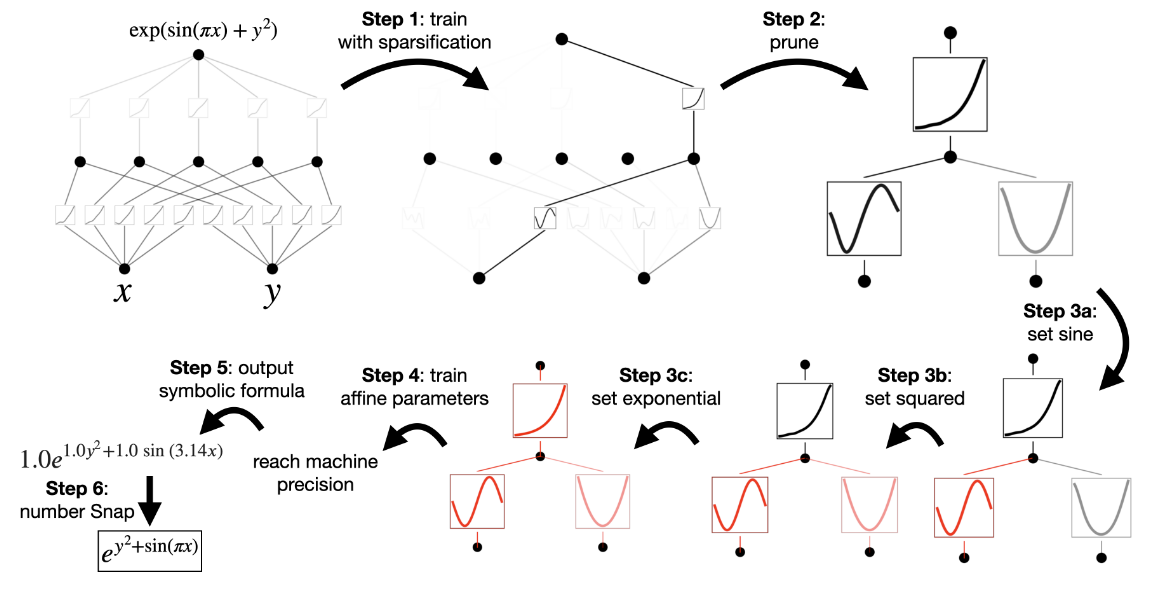
\includegraphics[height=0.8\textheight]{../images/kan_training.png}
	\end{figure}
	
\end{frame}

%------------------------------------------

\begin{frame}{Limitations of KANs}
	\begin{itemize}
		\item \textbf{Parameter \& memory blow-up.} For comparable width, KAN layers require substantially more parameters and activations than FC layers; memory scales poorly with $I,O,B$ and grid/spline settings $(G,k)$.
		\item \textbf{Convergence to sharp minima.} Hessian spectrum analyses show KANs tend to sharper minima $\Rightarrow$ weaker generalization (vision benchmarks).
		\item \textbf{Underperformance at scale.} On SciML (Neural ODEs), vision (Mixer/DeiT), and operator learning (FNO), KANs typically underperform MLPs despite higher cost.
		\item \textbf{Runtime/feasibility.} Longer training times and frequent OOM at moderate batch sizes on 16nB nPUs when scaling depth/width.
	\end{itemize}
\end{frame}

%------------------------------------------

\begin{frame}{Limitations - Parameter Complexity}
	\textbf{Fully Connected (FC) layer} with $O$ outputs and $I$ inputs:
	$$O \times (I+1)$$
	
	\textbf{KAN layer (B-spline)} with two shortcut weights, grid size $G$, $k$-order:
	$$I \times O \times (\,2 + G + k\,)$$
	
	Even ``width-matched'' KANs are often an order of magnitude larger than FC/MLP layers.
\end{frame}

%------------------------------------------

\begin{frame}{Limitations - Memory Footprint (Training)}
	\textbf{Fully Connected (FC) layer} accounting for both \textcolor{blue}{forward} and \textcolor{red}{reverse} pass (one matrix each), and the coefficients (parameters):
	$$
	\textcolor{blue}{O \times B} + \textcolor{red}{O \times B} + O \times (I+1)
	$$
	
	\textbf{KAN layer (B-spline)}
	$$
	\textcolor{blue}{I \times (1{+}G{+}k) \times B} 
	\;+\; \textcolor{red}{I \times (G{+}k{-}1) \times B} 
	\;+\; I \times O \times (2{+}G{+}k)
	$$
	
	KANs allocate extra tensors for B-spline evaluation and De Boor recursion.
\end{frame}

%------------------------------------------

\begin{frame}{Limitations - Convergence \& Generalization}
	\begin{itemize}
		\item Large-batch training tends to \emph{sharp} minima (many large positive eigenvalues); \emph{flat} minima correlate with better generalization.
		\item Empirically, KAN variants show Hessian spectra with \textbf{more positive eigenvalues} than MLP counterparts, \emph{even at small batches}.
		\item \textbf{Effect:} test-time accuracy lags behind MLPs on vision tasks; e.g., DeiT on CIFAR-100 shows $\sim$8--12\% lower Top-1 for B-spline KANs with \textbf{more} parameters.
	\end{itemize}
\end{frame}

%------------------------------------------

\begin{frame}{Empirical Evidence Across Domains}
	\textbf{Neural ODEs (SciML).}
	\begin{itemize}
		\item On Lotka–Volterra, Pleiades, Spiral ODE, KAN-ODEs reach \textbf{higher final loss}; MLP-ODEs fit dynamics better.
	\end{itemize}
	
	\textbf{Computer Vision.}
	\begin{itemize}
		\item MLP-Mixer/Conv-Mixer/DeiT: KAN variants converge to \textbf{sharper minima} and \textbf{lower accuracy}; parameter counts are 2--3$\times$ higher for KANs at similar or worse accuracy.
	\end{itemize}
	
	\textbf{Operator Learning (FNO).}
	\begin{itemize}
		\item Replacing lift/projection MLPs with KANs yields \textbf{slightly worse} test loss without residuals; with residuals, small gains appear but at \textbf{prohibitive memory cost}.
	\end{itemize}
\end{frame}

%------------------------------------------

\begin{frame}{References}
	\nocite{liu_kan_2025}
	\nocite{pal_understanding_nodate}
	\printbibliography[heading=none]
\end{frame}

\end{document}
